\chapter{Results}
\label{Results}

This chapter presents a comprehensive evaluation of the classification performance for the models applied in this study, with a focus on comparing the CatBoost and Graph Attention Network (GAT) models under varying layer configurations. Given the dataset's imbalance, multiple performance metrics are reported to provide a more nuanced assessment than accuracy alone.

\section{GAT vs. CatBoost Classification Performance}
\label{sec:gat_vs_catboost}

The performance of each model in predicting flight delays due to holding maneuvers was assessed using the following metrics:

\begin{itemize}
    \item \textbf{Accuracy}: Measures the overall proportion of correct predictions across all instances. While accuracy is a useful baseline metric, it can be misleading with imbalanced datasets, as it may remain high even if the model fails to correctly predict instances of the minority class, such as delayed flights.

    \item \textbf{Precision}: Represents the ratio of true positive predictions (correctly predicted delays) to all positive predictions made by the model. Precision provides insight into the model's ability to accurately identify actual delays, where higher precision indicates fewer false positives.

    \item \textbf{Recall}: The ratio of true positive predictions to the total number of actual positive instances (delays) in the dataset. A high recall indicates the model’s effectiveness in capturing most delayed flights, crucial in applications where missing delay predictions could impact operations.

    \item \textbf{F1-Score}: The harmonic mean of precision and recall, which balances these two metrics into a single score. The F1-score is particularly useful for imbalanced datasets, as it considers both false positives and false negatives, providing a balanced measure of performance.
\end{itemize}

The performance of each model configuration across these metrics is shown in Table \ref{tab:gat_catboost_metrics}, highlighting the trade-offs between model complexity (number of GAT layers) and classification effectiveness. Notably, the CatBoost model achieves balanced performance, which is advantageous given the imbalanced dataset.

\begin{table}[!htbp]
	\centering
	\caption{Performance metrics for various GAT layer configurations and CatBoost with graph features.}
	\label{tab:gat_catboost_metrics}
	\begin{tabular}{ccccc}
		\toprule
        \textbf{Model} & \textbf{Test Accuracy} & \textbf{Precision} & \textbf{Recall} & \textbf{F1-Score} \\
		\midrule
        \textbf{CatBoost} & 0.91 & \textbf{0.10} & 0.56 & \textbf{0.17} \\
        \textbf{1 GAT Layer} & \textbf{0.95} & 0.03 & 0.06 & 0.04 \\
        \textbf{3 GAT Layers} & 0.52 & 0.01 & 0.40 & 0.03 \\
        \textbf{5 GAT Layers} & 0.57 & 0.01 & 0.30 & 0.02 \\
        \textbf{10 GAT Layers} & 0.91 & 0.02 & 0.08 & 0.03 \\
        \textbf{30 GAT Layers} & 0.02 & 0.02 & \textbf{0.99} & 0.03 \\
		\bottomrule
	\end{tabular}%
\end{table}


As we can see, Catboost outperforms GAT in terms of precision and F1-Score, while GAT models with more layers tend to have higher recall and with a single layer the higher accuracy. However, the 30-layer GAT model exhibits a significant drop in accuracy, indicating overfitting. The CatBoost model, with a balanced performance across all metrics, is better suited for the imbalanced dataset, as it captures both delayed and non-delayed flights effectively.

Since we are dealing with an unbalanced setting, it was already expected that the CatBoost model would perform better, as it is a decision tree ensemble model that is known for its robustness in handling class imbalance. That is why it had the higher F1-score that is in our problem the most reliable metric, since we want to predict holding and it's better to be wrong some times than always predict `no holding'. The GAT model, on the other hand, as most of GNNs have trouble in dealing with class imbalance, as they tend more to overfitting.

\section{Predictive Regression Analysis and Interpretability}

Beyond classification, we extended our investigation to evaluate the CatBoost model's capacity for regression on continuous delay values and its interpretability. The objective was to assess how effectively CatBoost could predict the extent of flight delays while providing insights into which features were most influential in the model's decision-making. This section explores both aspects—interpretability and regression accuracy—with a focus on the model’s performance and its potential operational impact.

\subsection{Interpretability of the CatBoost Model}

One of the major advantages of the CatBoost model is its transparency, particularly when compared to more complex neural network architectures. By utilizing graph-based features, CatBoost not only achieved favorable classification performance but also provided a clearer view of feature importance. Unlike black-box models, CatBoost can be examined through Explainable AI (XAI) techniques, which help interpret how specific features contribute to predictions.

Figure \ref{fig:catboost_feature_importance} presents the feature importance for the CatBoost model, identifying which graph-based features most significantly influence the prediction of flight delays due to holding maneuvers. This insight confirms the utility of graph-based features in providing a robust predictive foundation and highlights their relative impact on the delay predictions.

\begin{figure}[!htbp]
    \centering
    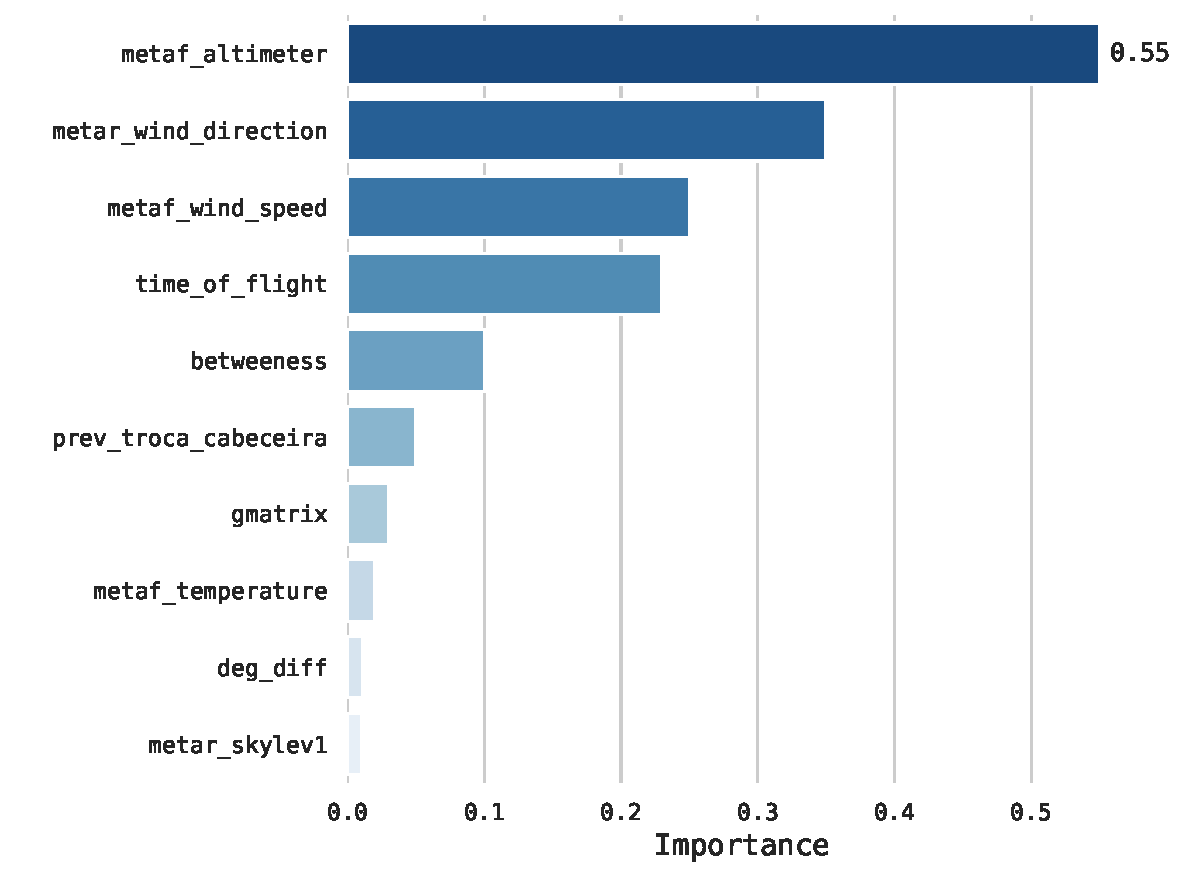
\includegraphics[width=0.8\textwidth]{img/feature_importance_plot.pdf}
    \caption{Feature importance for the CatBoost model on the airport network dataset, indicating the relevance of graph-based features.}
    \label{fig:catboost_feature_importance}
\end{figure}

\subsection{Regression Performance}

To further assess the model's robustness, we applied CatBoost to a regression task, predicting continuous delay values rather than binary classifications. Figures \ref{fig:y_pred} and \ref{fig:y_test} display the distribution of predicted ($y_\text{pred}$) and actual ($y_\text{test}$) delay values, respectively. By comparing these distributions, we gain insights into CatBoost’s ability to capture trends and variability within the dataset.

\begin{figure}[!htbp]
    \centering
    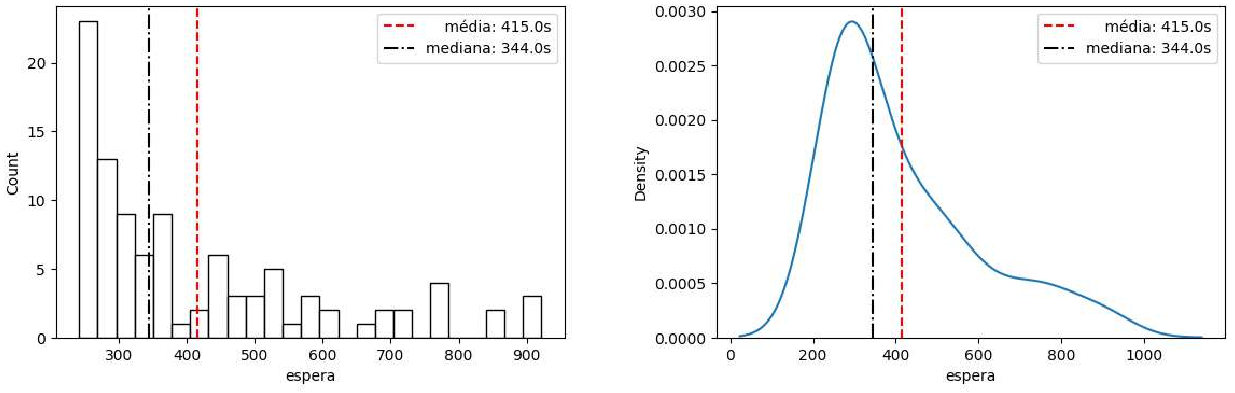
\includegraphics[width=0.8\textwidth]{img/regression_catboost_ypred.pdf}
    \caption{Predicted delay values distribution ($y_\text{pred}$) for the regression task using CatBoost.}
    \label{fig:y_pred}
\end{figure}

\begin{figure}[!htbp]
    \centering
    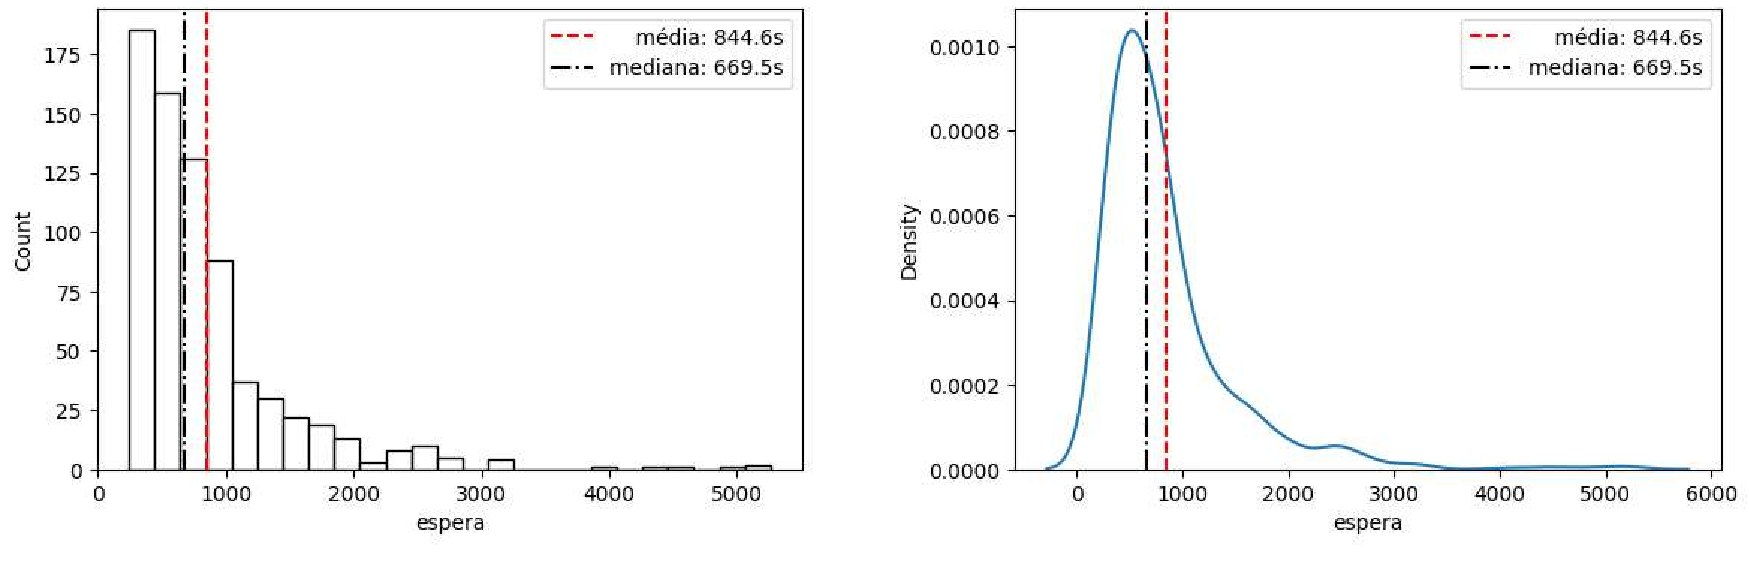
\includegraphics[width=0.8\textwidth]{img/regression_catboost_ytest.pdf}
    \caption{Actual delay values distribution ($y_\text{test}$) for the regression task in the test set.}
    \label{fig:y_test}
\end{figure}

The comparison between predicted and actual distributions reveals that CatBoost captures core trends in the data, though some deviation at extreme delay values suggests potential areas for improvement. Overall, CatBoost’s performance in regression further validates its flexibility and predictive power, offering a promising model for continuous delay predictions in airport network analysis.

\section{Deployment and Implementation}

The source code for this project is available on GitHub at \href{https://github.com/graph-learning-ita/airnet-holding-ml/}{https://github.com/graph-learning-ita/airnet-holding-ml/}.

We have also developed a web-based simulation tool using Folium and Streamlit, which visualizes flight delays as predicted by the CatBoost model. Users can specify a simulation period, during which the model's predictions guide the flight paths and indicate holding maneuvers in real time, enabling stakeholders to observe potential delay scenarios. This interactive platform enhances the practical application of the model by providing a visual, user-friendly interface to interpret predictions dynamically.

We called the application `Airdelay' and it is available at \url{https://airdelay.manoel.dev}. Figure \ref{fig:airdelay} shows a screenshot of the Airdelay tool, illustrating the predicted flight delays due to holding maneuvers. Users can interact with the map, explore different scenarios, and observe the model's predictions in real time, enhancing their understanding of the model's performance and potential operational impact.

\begin{figure}
    \centering
    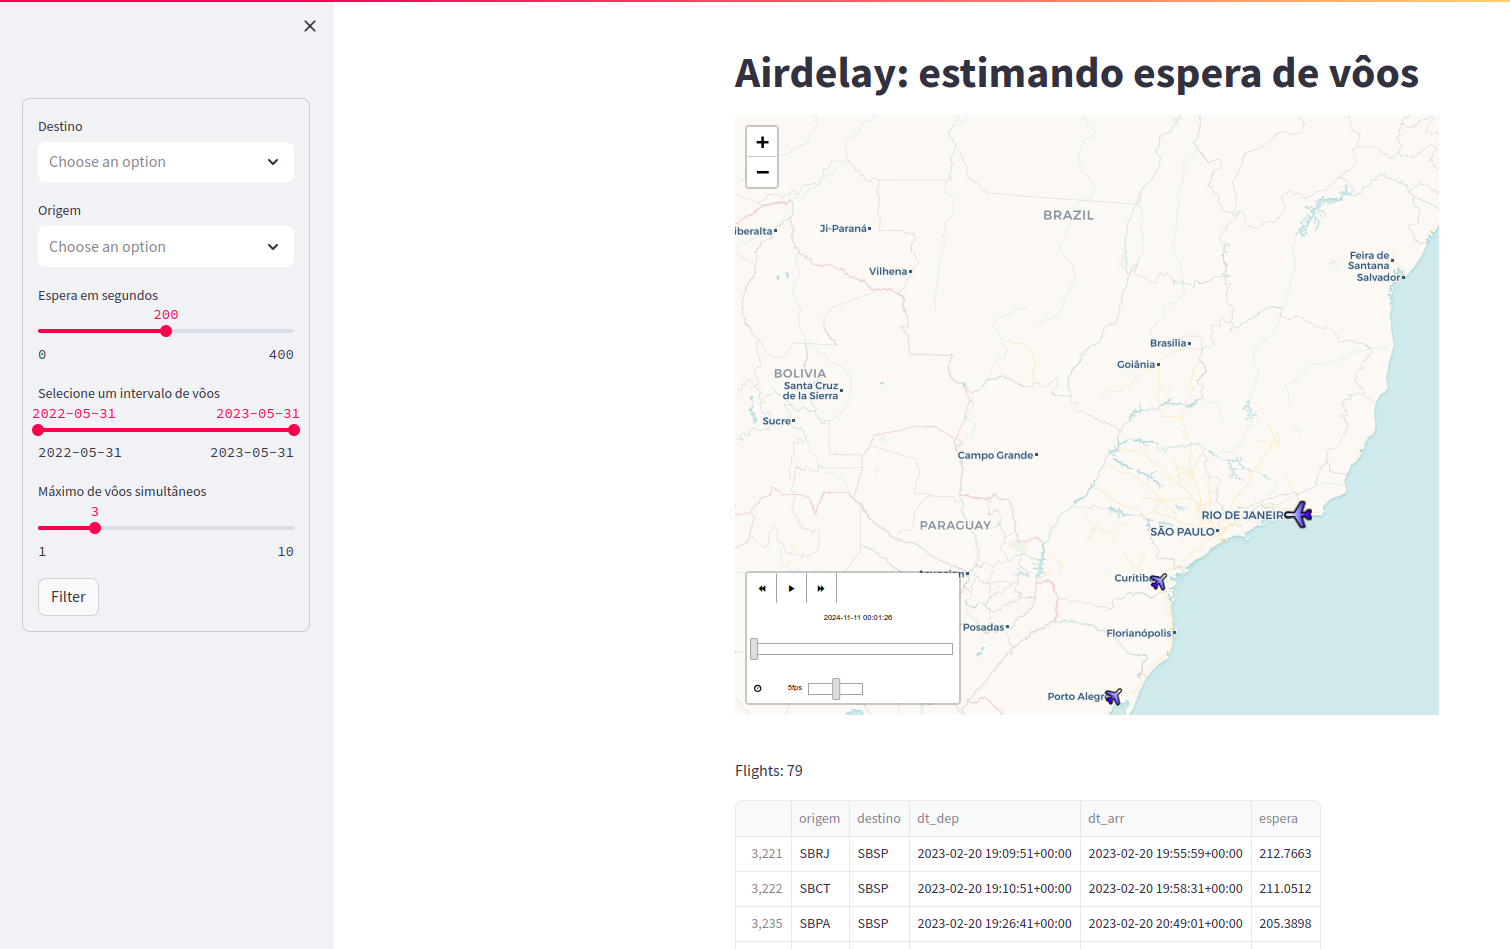
\includegraphics[width=0.8\textwidth]{img/airdelay.png}
    \caption{Airdelay web-based simulation tool, showing predicted flight delays due to holding maneuvers.}
    \label{fig:airdelay}
\end{figure}

\section{Discussion, Limitations and Future Works}

The results presented in this chapter provide insights into the trade-offs between the CatBoost model and various GAT configurations. CatBoost, with its interpretable, tabular-focused approach, offers a more reliable model for imbalanced data, outperforming GAT in both precision and recall. GAT models with additional layers did not significantly improve performance and, in some cases, led to overfitting or instability due to the network's complexity and the dataset's limitations.

By employing graph features in a gradient boosting framework, we have shown that structured data representations, combined with graph-theoretic metrics, can in some cases outperform GNNs in predictive tasks. Revealing that traditional graph machine learning continues important even in the area of graph deep learning, because of the possibility of integrating graph measures into tree-based models.

However, our work is limited due to the lack of time for more extensive hyperparameter tuning and model optimization. Future work should focus on refining the GAT model architecture, exploring additional graph-based features, and addressing the dataset's class imbalance more effectively with undersampling and/or oversampling techniques. Additionally, other ML models, such as SVM, could be tested.

Furthermore, there are new GNN architectures that could be explored. A recent work by \citeonline{egressy2024provably} introduced a provably powerful graph neural network for directed multigraphs, that could improve minority-class F1 score by up to 30\% in their tests. In our scenario this could be a game changer, since the problem with the GAT model was the class imbalance.
